\documentclass{article}
\usepackage[utf8]{inputenc}
\usepackage{graphicx}
\usepackage{hyperref}
\author{Felix Bello, Gilles Brunner}
\title{Arbeitsauftrag 2}
\begin{document}
	\maketitle
	\section{Einführung}
Nachstehend wird beschrieben, wie wir für eine Wordpress-Installation im Rahmen des Moduls IKS vorgehen. Da wir die Aufgabe auf unserem Debian-Server lösen, gibt es einige Unterschiede bei gewissen Namen: Apache ist nicht unter httpd zu finden, sondern Apache2 und Benutzer und die Gruppe für unseren Webpfad ist www-data (das nur als Info, damit ist kein Durcheinander gibt bei der Aufführung unsere Pfade und 	Benutzerberechtigungen.)
	\section{LAMP}
	\textit{lucy:/home/gilles\# screen -S newScreen}
	\newline
	\textit{lucy:/home/gilles\# apt-get install mariadb-client-10.0 mariadb-server-10.0 apache2 apache2-doc php5 php5-mysql libapache 2-mod-php5}
	\newline
	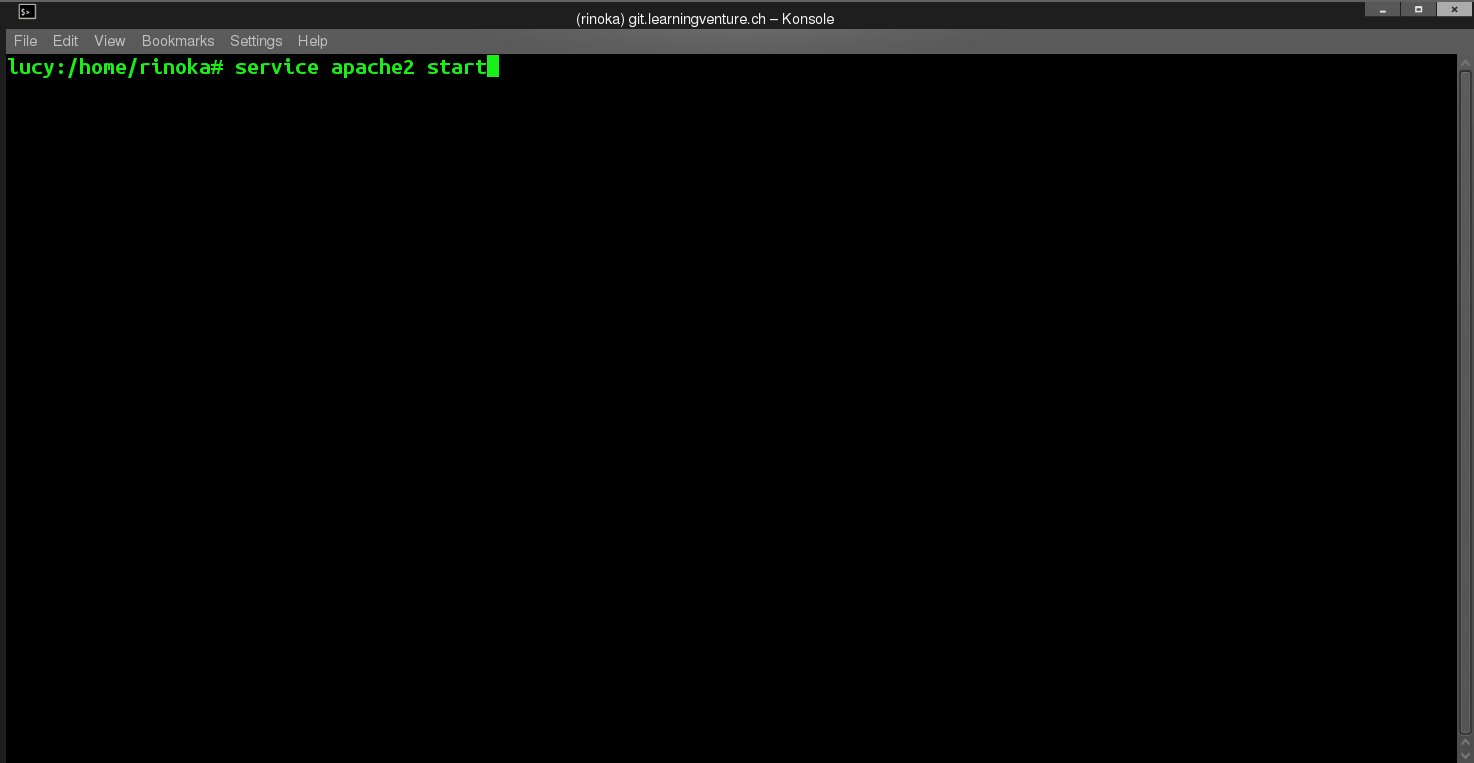
\includegraphics[width=13cm]{../Pics/start_apache}
	\newline
	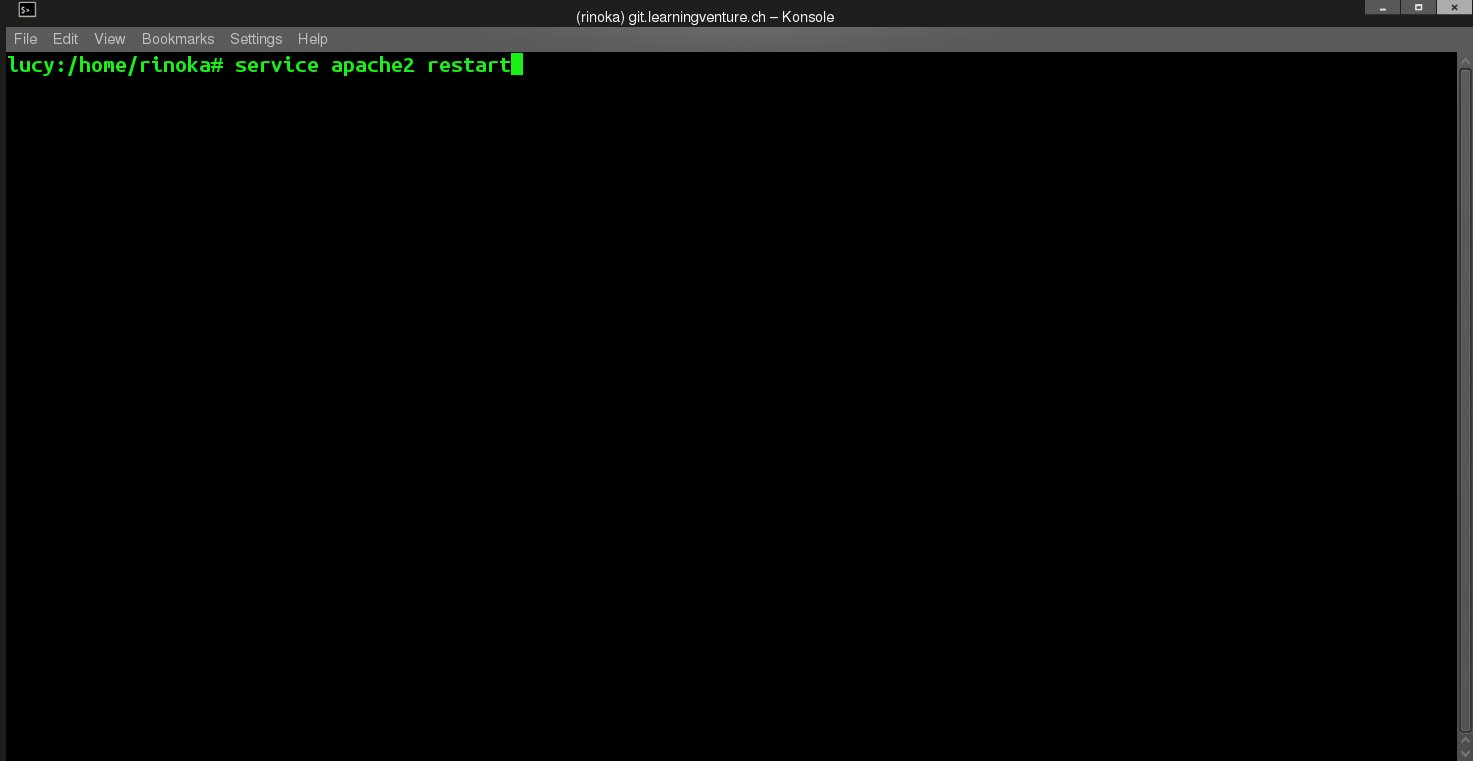
\includegraphics[width=13cm]{../Pics/apach2restart}
	\newline
	\subsection{Linux}
	\subsection{Apache}
	Gemäss der im Auftrag erfordlichen Konfigurationsdateien muss die Wordpress-Installation auf dem Server unter folgendem Dateipfad installiert werden: /var/www/html/wordpress.
	Allerdings soll Wordpress auf IP-Adresse/blog aufgerufen werden. Dazu muss der VirtualHost in /etc/apache2/sites-available/ angepasst werden.
	\subsection{VirtualHost}
	Die Dokumentation, die wir uns für die erforderliche VirtualHost-Konfiguration angeschaut haben, befindet sich hier: \url{https://httpd.apache.org/docs/2.2/mod/mod_alias.html\#alias}
	Die Idee ist folgende:
	The directives contained in this module allow for manipulation and control of URLs as requests arrive at the server. \underline{The Alias} and \underline{ScriptAlias} directives are used to map between URLs and filesystem paths.
	Das heisst, dass man mit einer bestimmten URL (in unserem Falle IP-adresse/blog) auf einen bestimmten Pfad auf dem Server selbst zugreifen kann (in unserem Falle /var/www/html/wordpress). Dazu muss die VirtualHost- Konfigurationsdatei in /etc/apache2/sites-available/wordpress.conf entsprechend angepasst werden:
	\newline
	\newline
	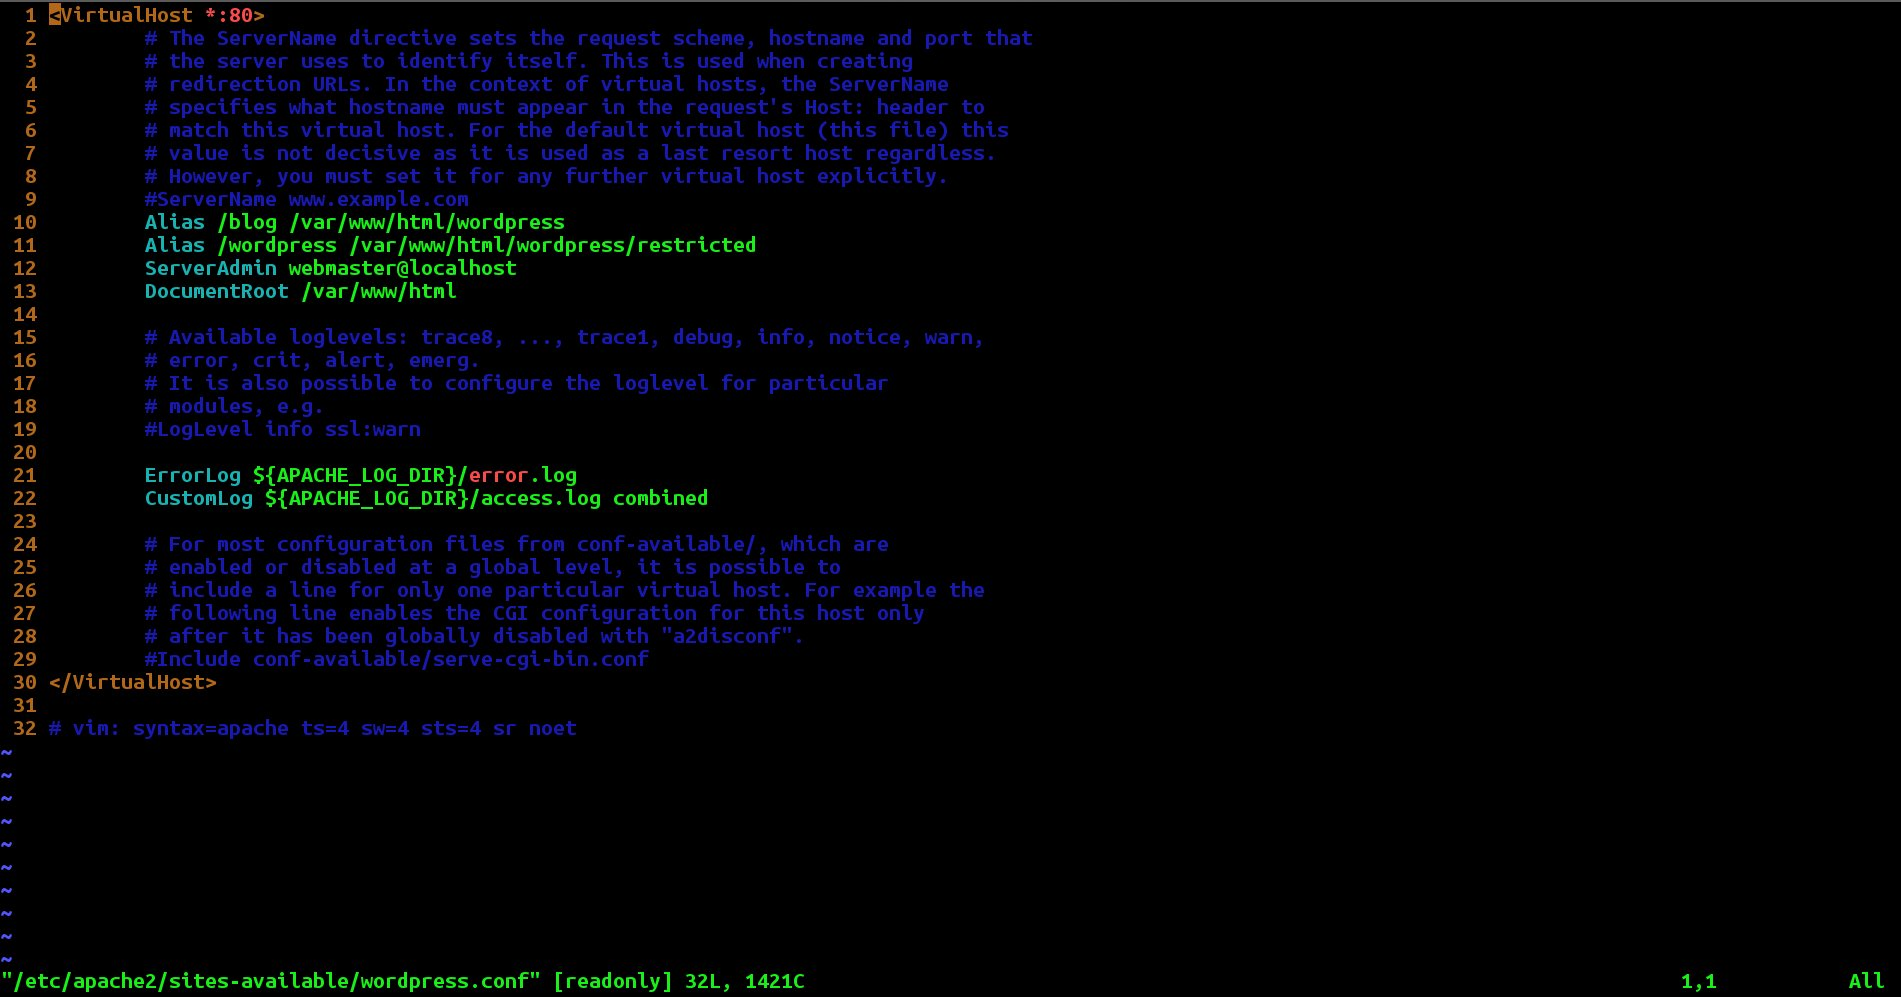
\includegraphics[width=13cm]{../Pics/wordpress}
	\newline
	\newline
	Die VirtualHost-Konfigurationsdatei befindet sich wie erwähnt in /etc/apache2/sites-available/
	Darin befindet sich am Anfang eine Standard-Konfigurationsdatei mit dem Namen:
	\begin{itemize}
		\item 000-default.conf
	\end{itemize}
	Nun brauchen wir eine also wordpress.conf. Dazu könnten wir einfach die bestehende Datei umbenennen (mv 000-default.conf wordpress.conf), aber wir haben uns entschieden, sie beizubehalten und einfach basierend auf der Default-Datei eine entsprechende wordpress.conf zu erstellen (cp 000-default.conf wordpress.conf). Wichtig ist nun zu beachten, dass nicht beide Konfigurationsdateien aktiviert sind. Um das zu testen, untersucht man den Ordner sites-enabled wie folgt:
	\begin{itemize}
		\item ls /etc/apache2/sites-enabled
	\end{itemize}
	Falls sich  000-default.conf darin befindet, deaktiviert man sie folgendermassen:
	\begin{itemize}
		\item a2dissite  000-default.conf
	\end{itemize}
	Der Grund dafür ist, wenn beide Konfigurationsdateien aktiviert sind (d.h. 000-default.conf und wordpress.conf) dann wird nur 000-default.conf verwendet, weil sie alphabetisch vor wordpress.conf kommt (das kann man testen, wenn man 000-default.conf deaktiviert und in sites-available folgendermassen umbenennt: x000-default.conf). Wenn man x000-default.conf und wordpress.conf beide aktiviert, wird dieses mal wordpress.conf verwendet, weil w vor x kommt (diese möchten wir nur am Rande anmerken, weil wir uns beim Testen kurz mit dieser Situation auseinandersetzen mussten).
	Wir haben also unser Alias gemäss der in der Dokumentation beschriebenen Syntax (Alias URL-path file-path|directory path) der VirtualHost Konfigurations-Datei /etc/apache2/sites-available/wordpress.conf hinzugefügt. Der Inhalt ist in Screenshot (Nr. X) zu sehen. Zusätzlich haben wir beschlossen, dass die IP-Adresse/wordpress nicht auf den Blog führen soll (es reicht, wenn man über /blog drauf kommt). Zu diesem Zweck haben wir eine index.html mit einer kleinen Nachricht definiert.
	\subsection{MariaDB}
	Wir haben uns wie bereits erwähnt für \textit{\textbf{MariaDB}}  als Datenbank entschieden, um diese zu Konfigurieren wird automatisch vom installer, den wir bereits ausgeführt haben mit \textit{\textbf{lucy:/home/gilles\# apt-get install mariadb-client-10.0 mariadb-server-10.0 apache2 apache2-doc php5 php5-mysql libapache 2-mod-php5}} die passwortabfrage angezeigt.
	\newline
	\newline
	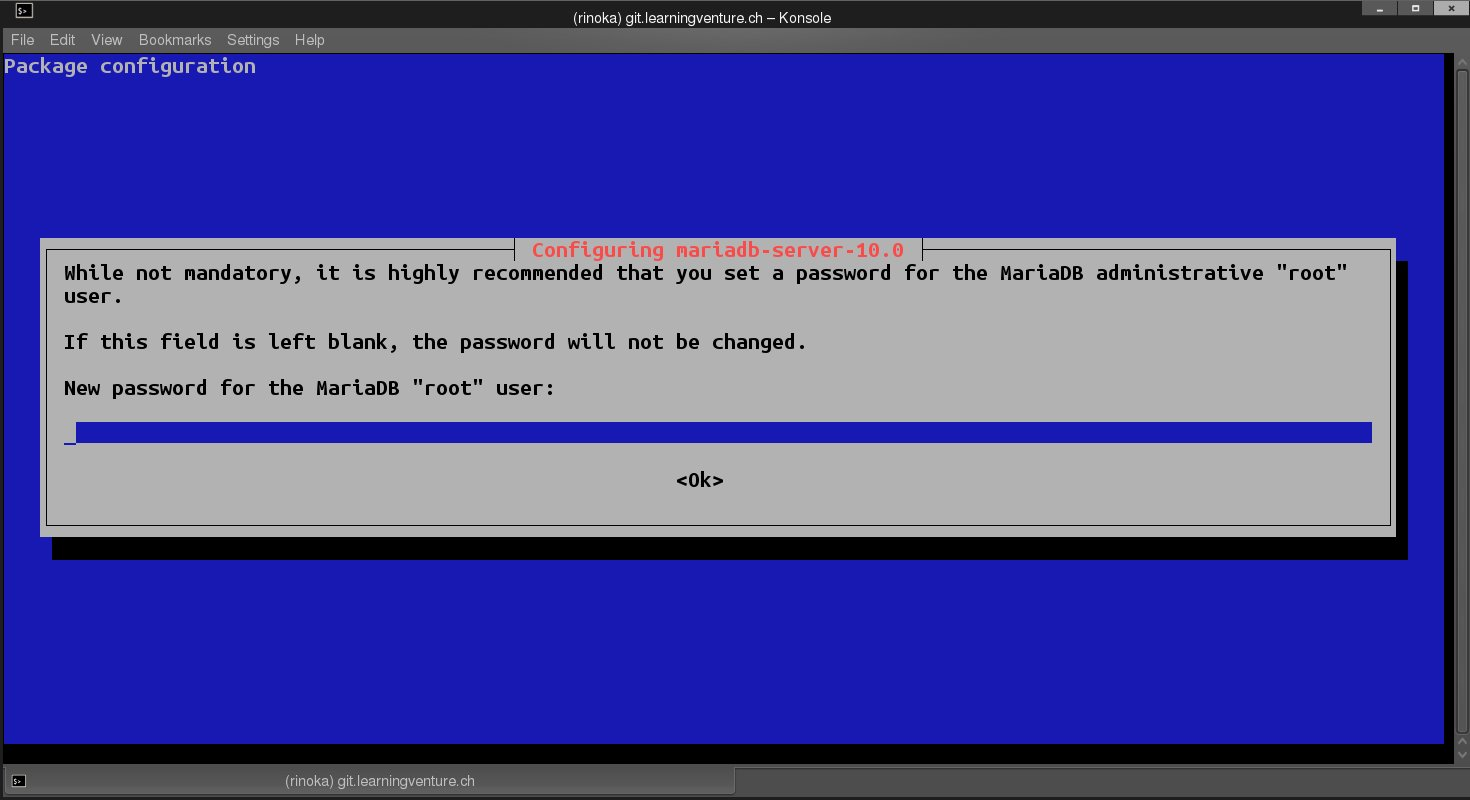
\includegraphics[width=13cm]{../Pics/3-lamp-stack-mariadb}
	\newline
	\newline
	Zunächst einmal müssen wir uns einloggen:
	\newline
	\textit{lucy:/var/www/html/wordpress\# mysql -u root -p}
	\newline
	Hat es geklappt sieht es wie folgt aus:
	\newline
	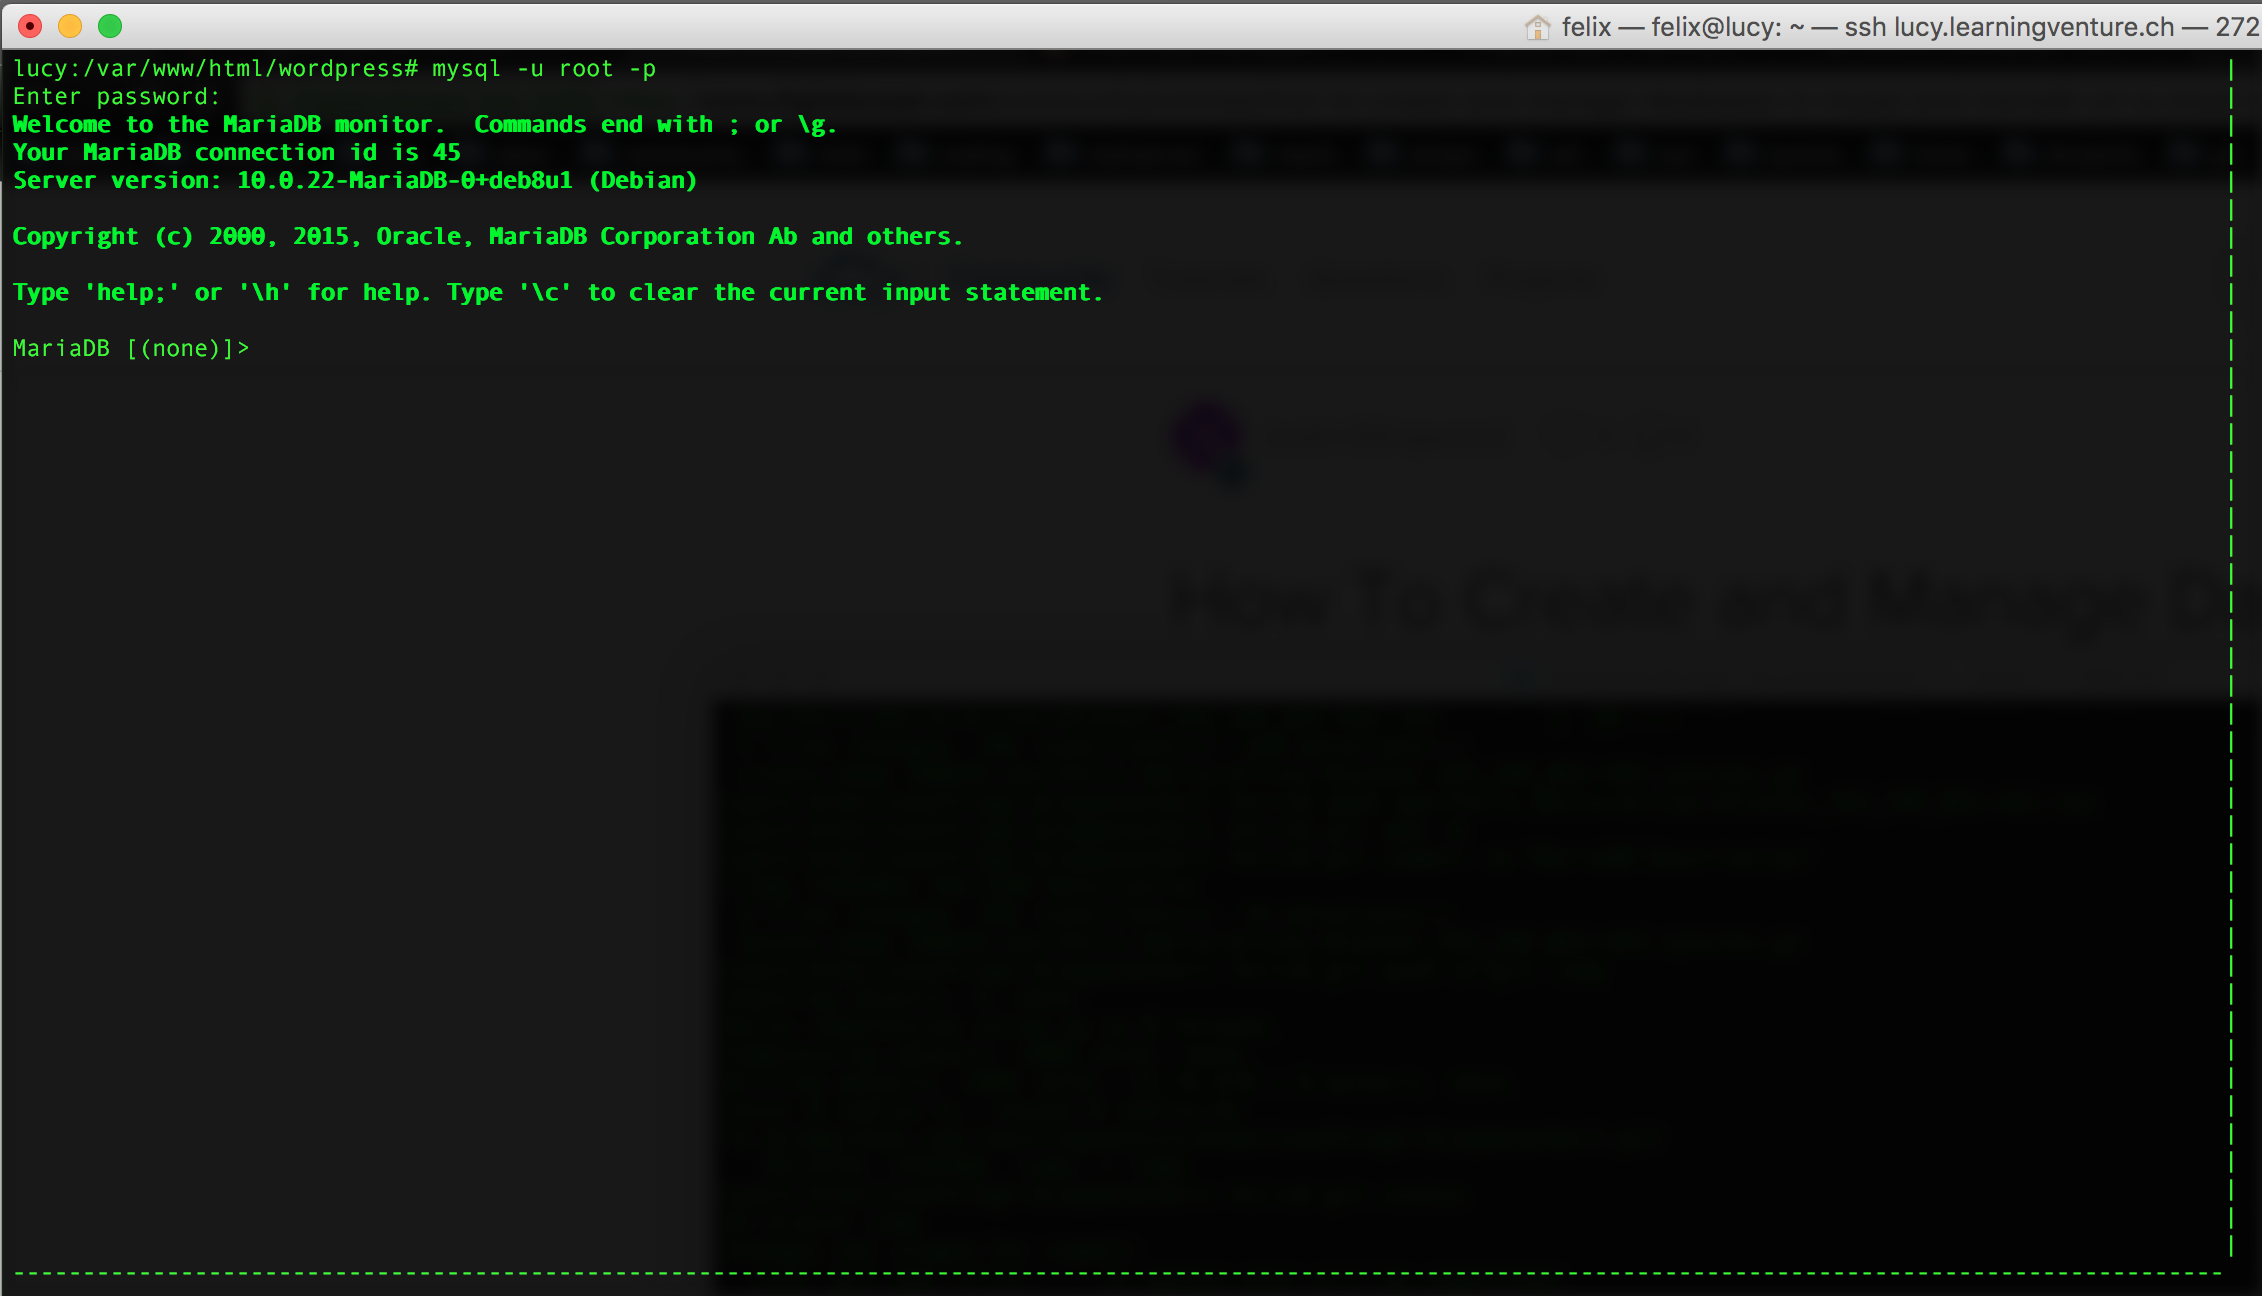
\includegraphics[width=13cm]{../Pics/21-maria-db-login-success}
	\newline
	Erstellen der Datenbank wie folgt mit folgendem befehl:
	\newline
	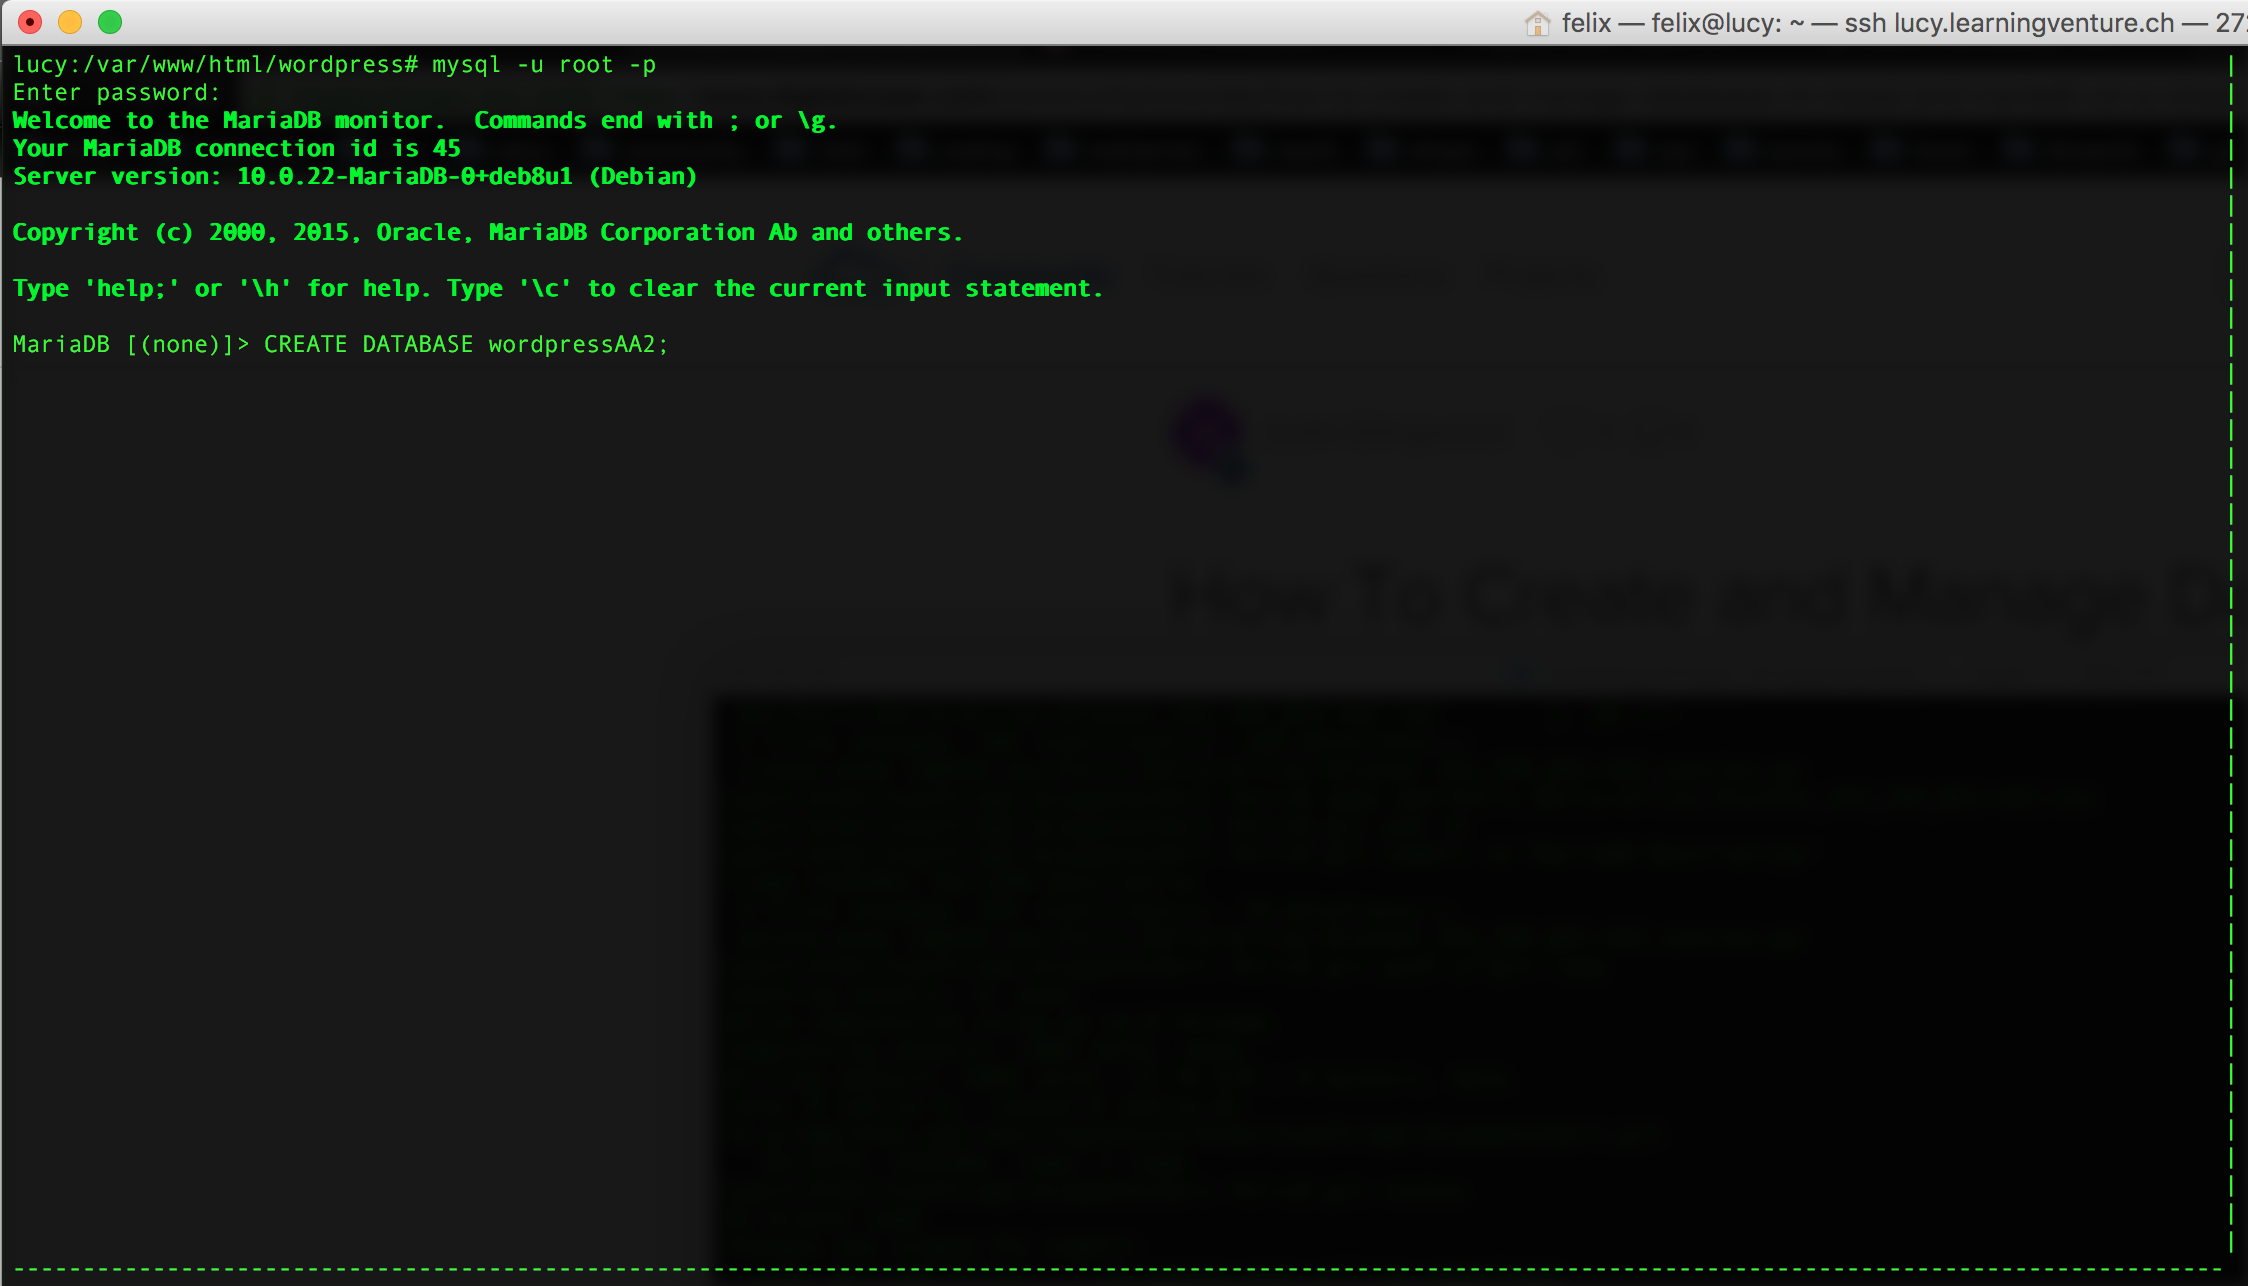
\includegraphics[width=13cm]{../Pics/22-maria-db-create}
	\newline
	Wenn diese erfolgreiche erstellt wurde:
	\newline
	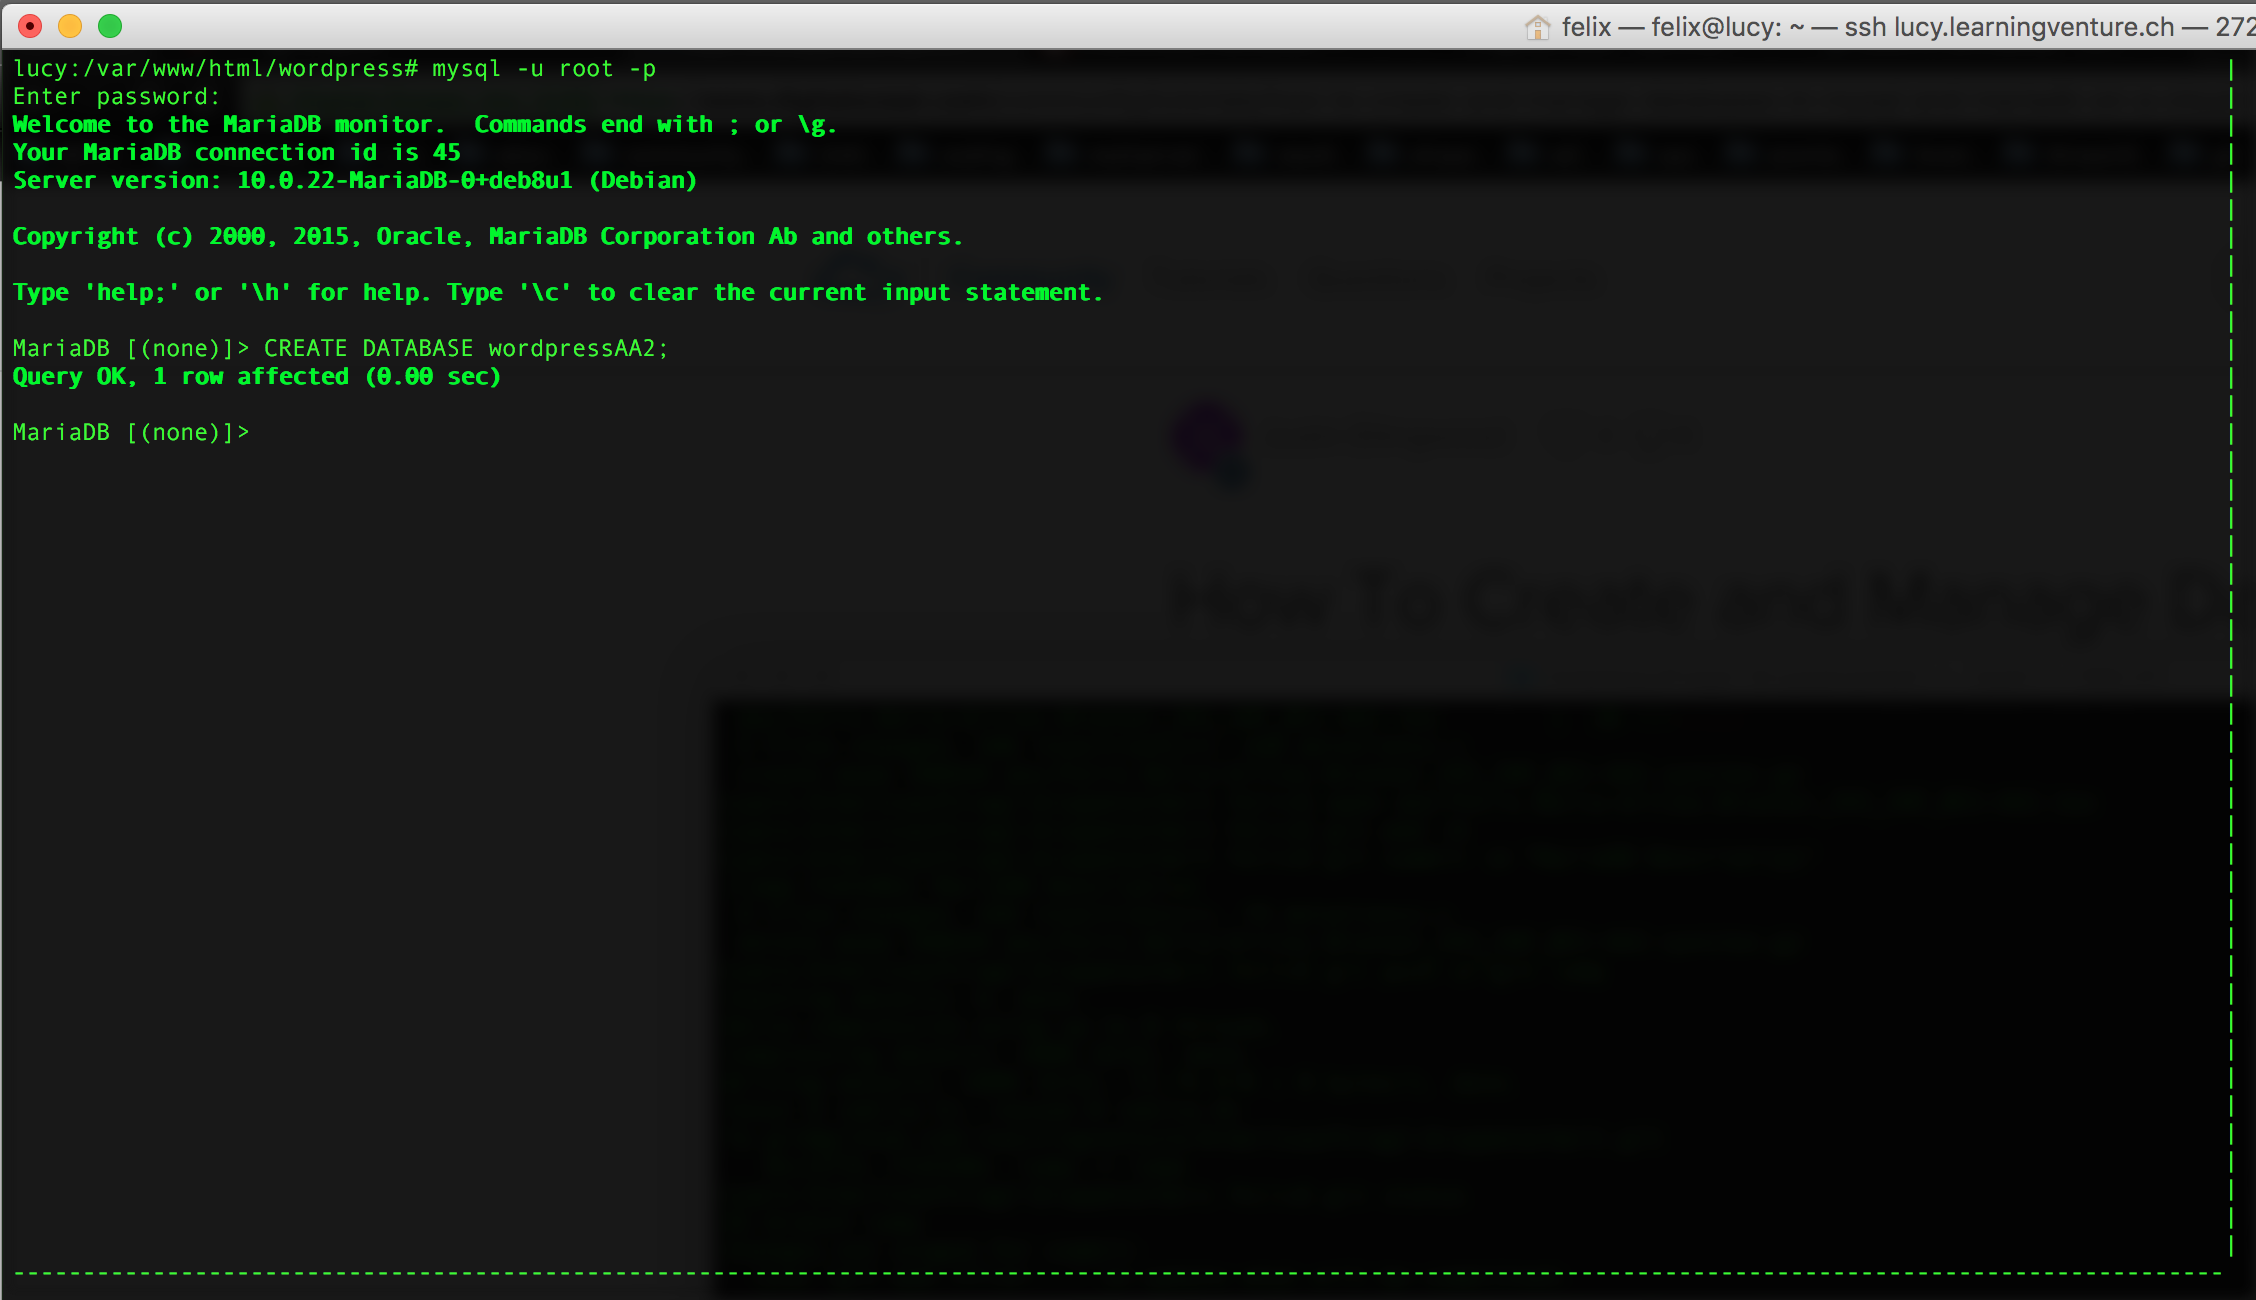
\includegraphics[width=13cm]{../Pics/23-maria-db-create-success}
	\newline
	Kontrolle ob diese auch erstellt wurde mit folgendem befehl:
	\newline
	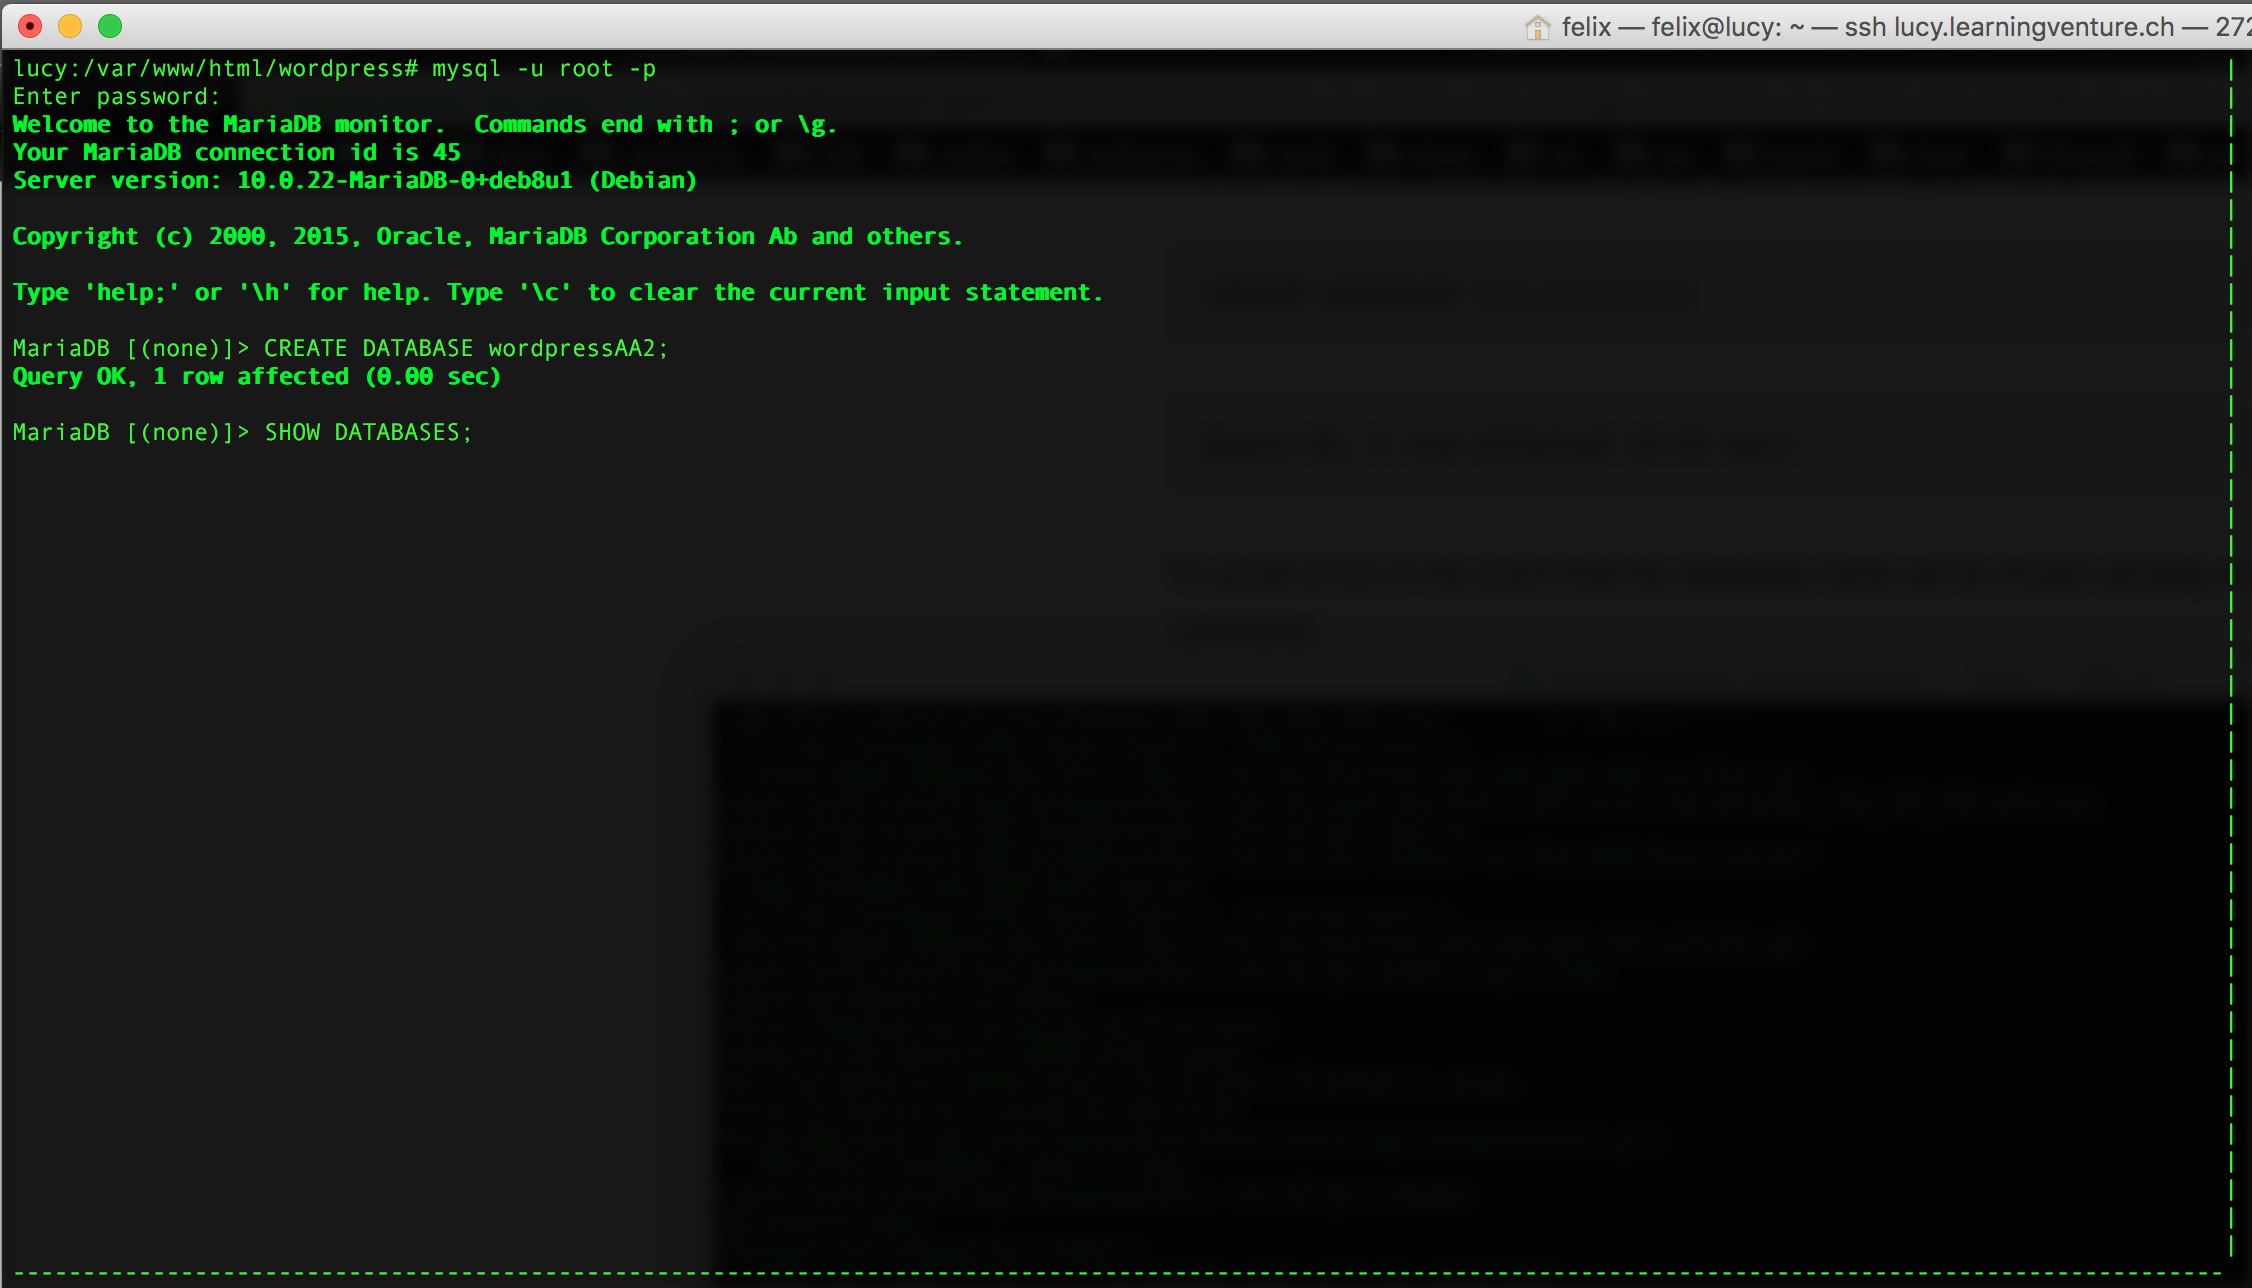
\includegraphics[width=13cm]{../Pics/24-maria-db-show}
	\newline
	Sieht es wie folgt aus, wurde die Datenbank erfolgreich erstellt:
	\newline
	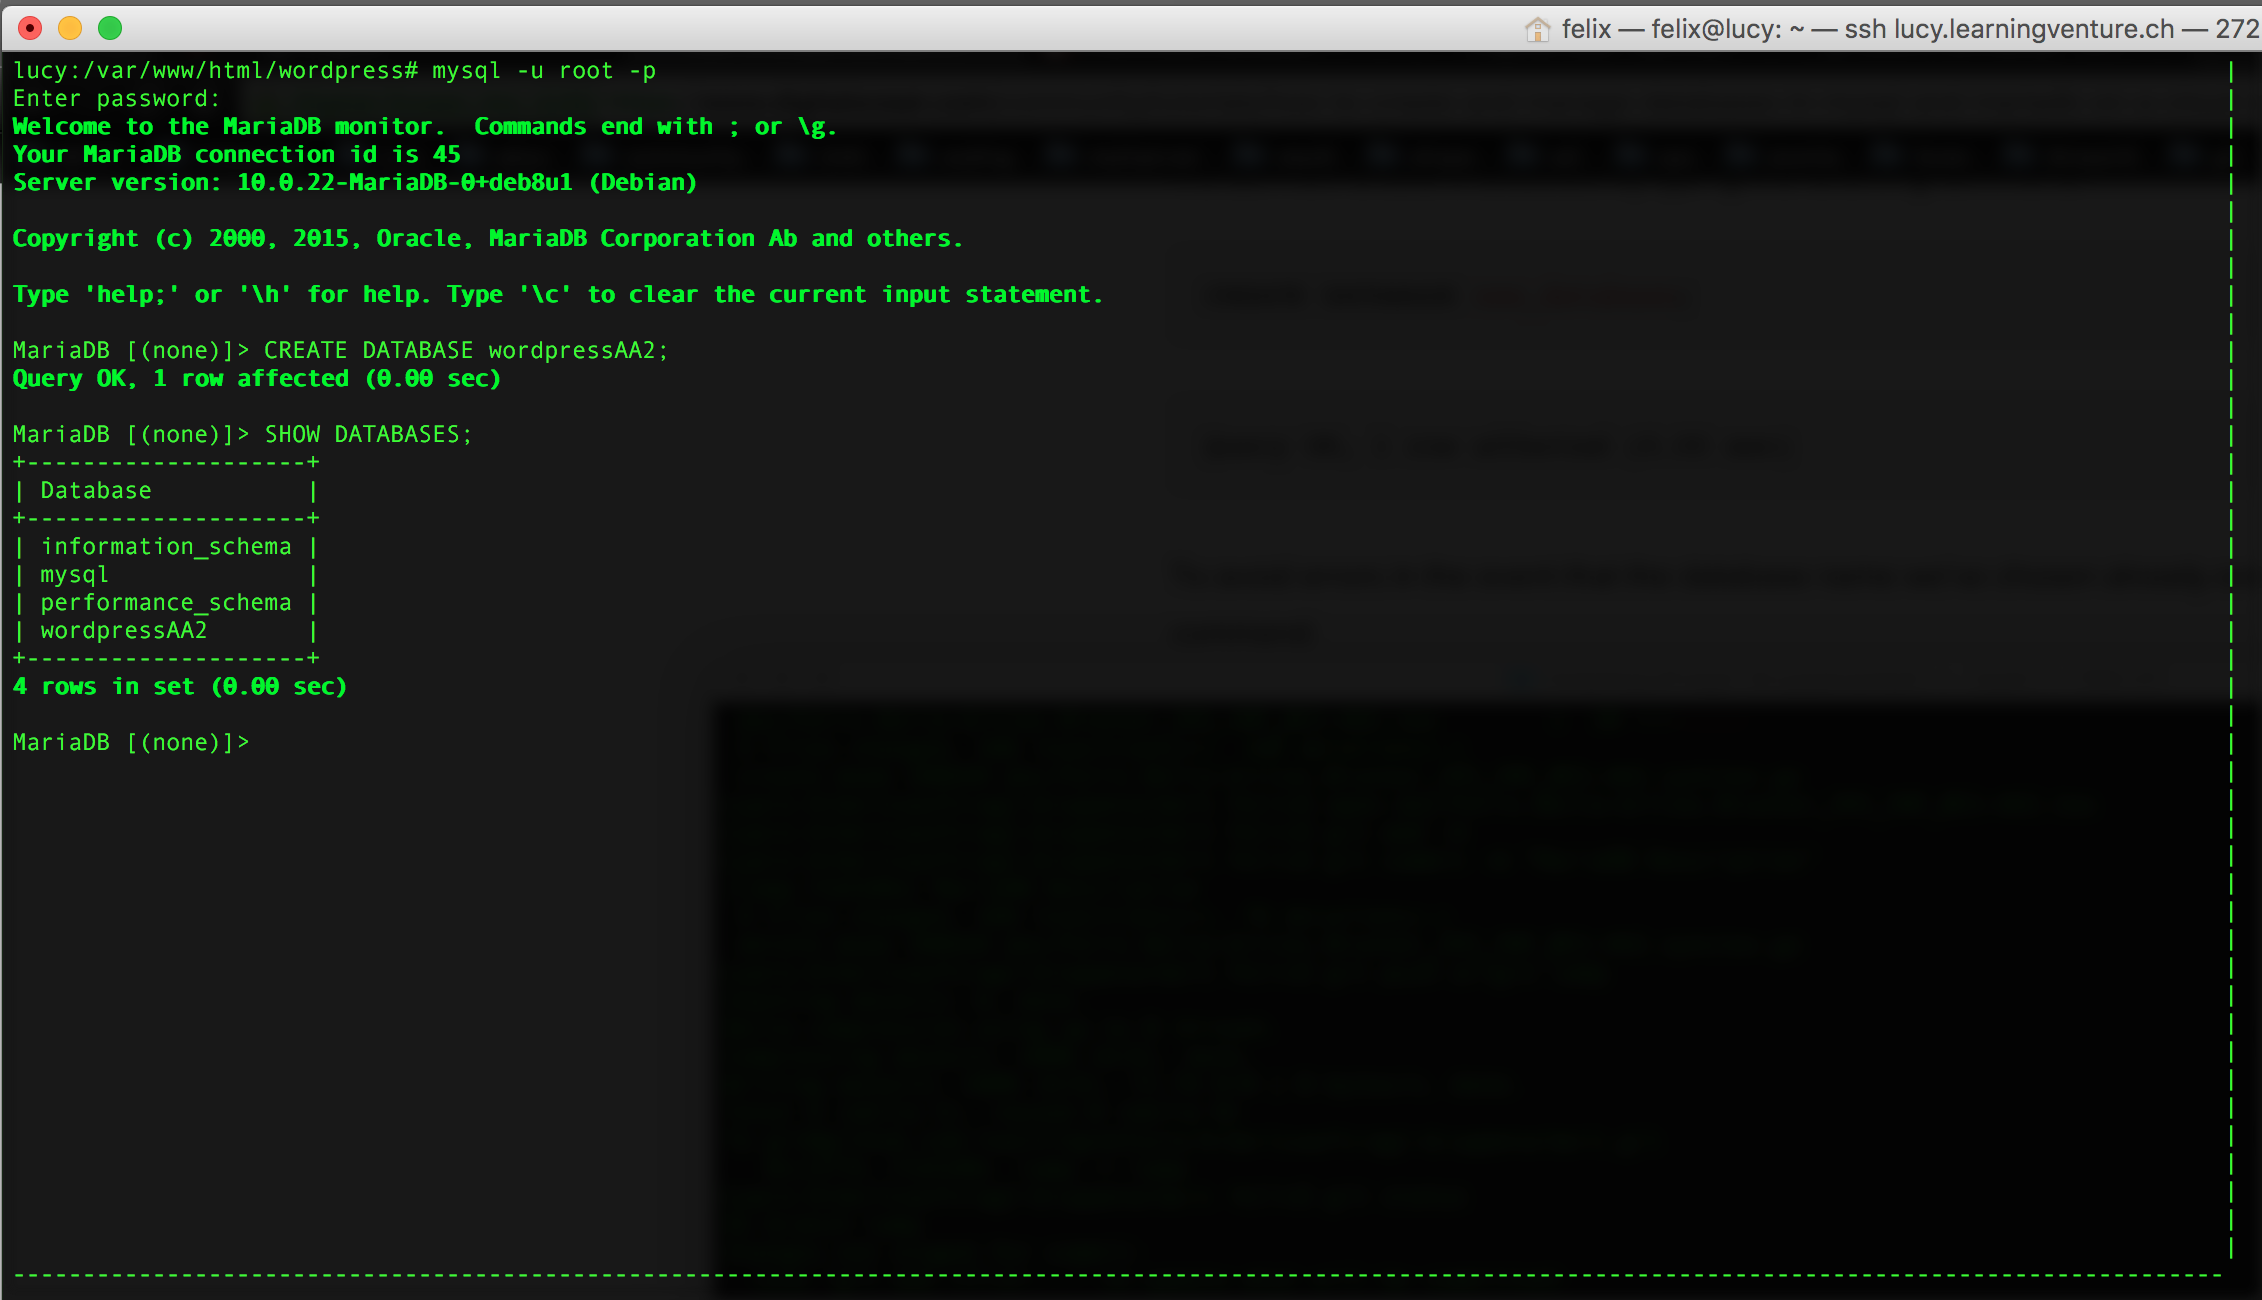
\includegraphics[width=13cm]{../Pics/25-maria-db-show-success}
	\newline
	Entsprechend kann man jetzt den MariaDB Admininterface verlassen mit:
	\newline
	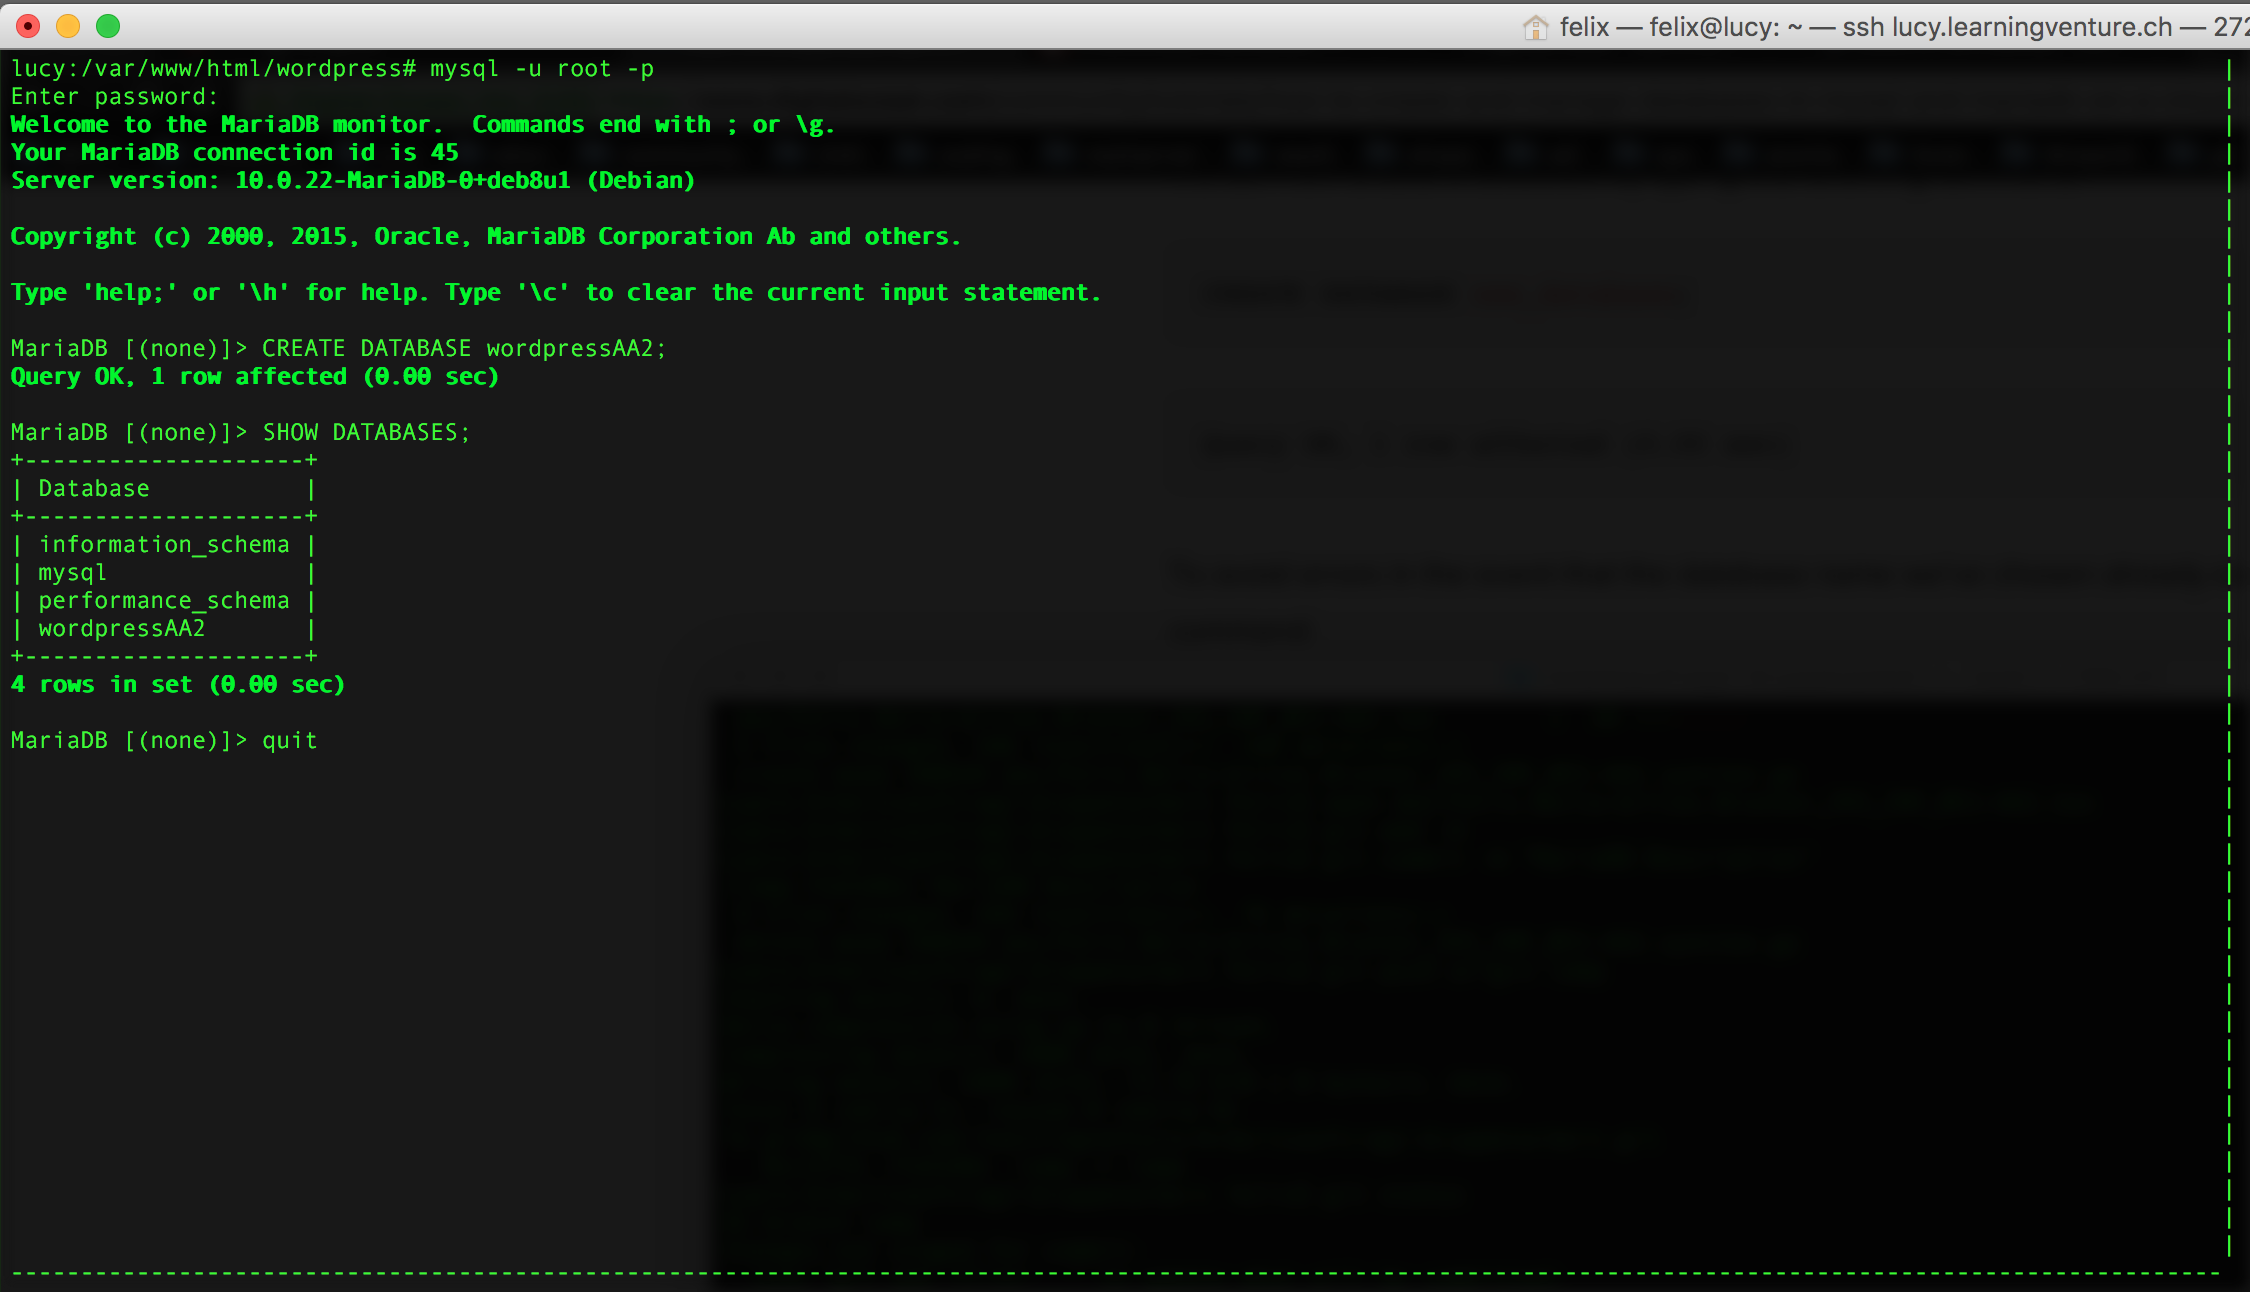
\includegraphics[width=13cm]{../Pics/26-maria-db-quit}
	\newline
	Wenn alles geklappt hat sieht es wie folgt aus:
	\newline
	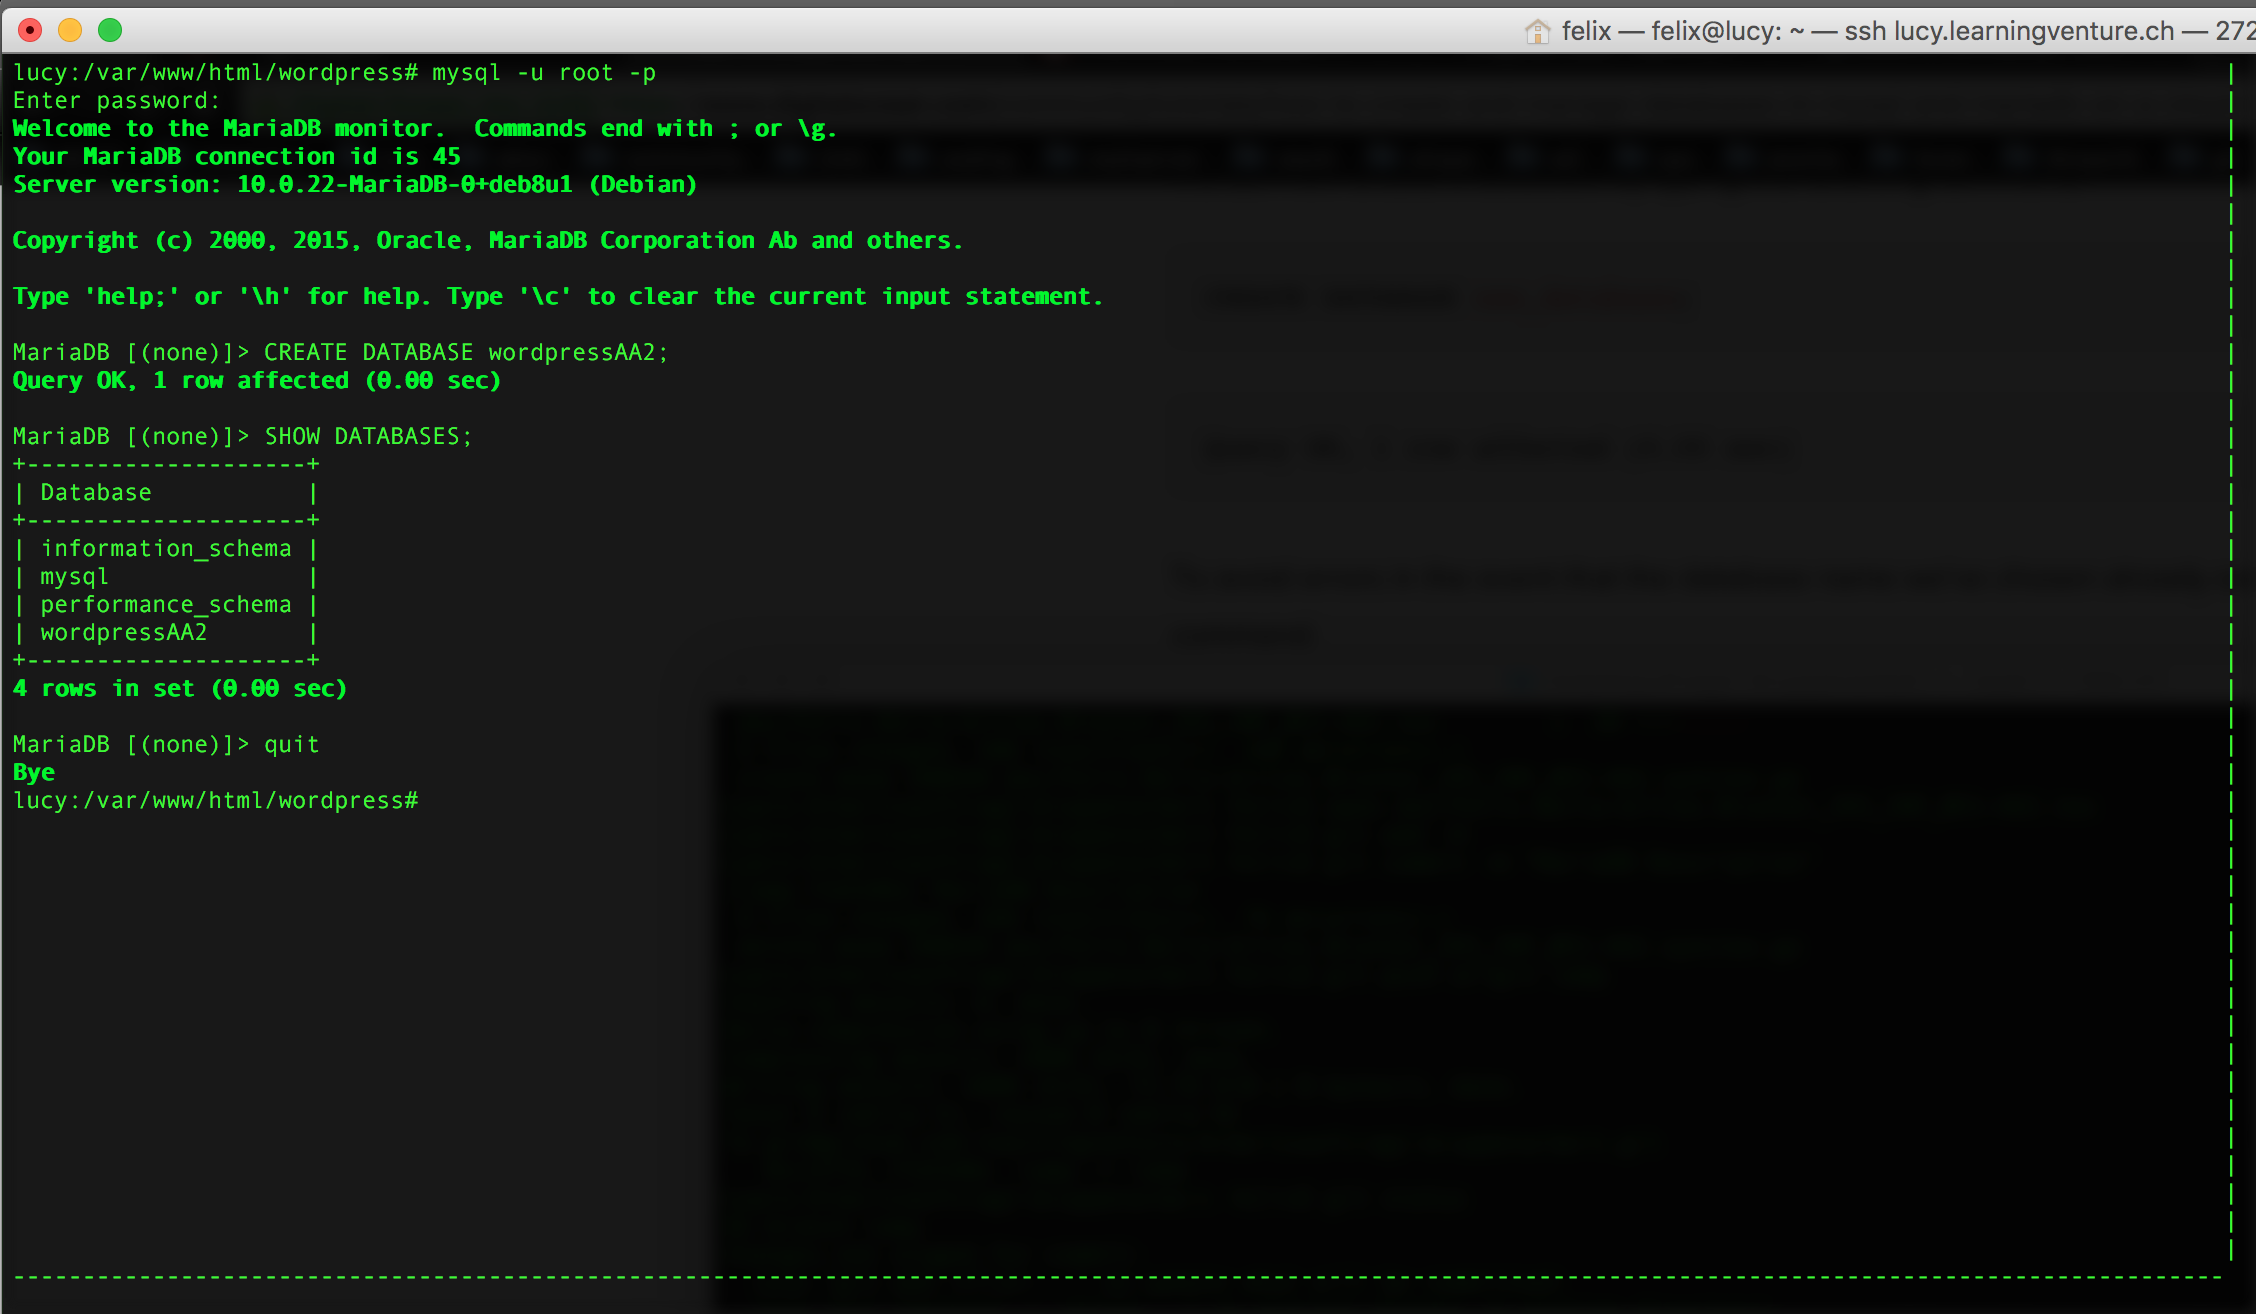
\includegraphics[width=13cm]{../Pics/27-maria-db-quit-success}
	\newline
	
	\subsection{PHP}
	\section{WordPress}
	\section{OwnCloud}
\end{document}